% Ergebnisse


\chapter{Ergebnisse}
\label{ergebnisse}

\todo[inline]{Wo Rendering zeigen? Qualität der Daten ansprechen?}

Das Ergebnis der Implementierung ist eine aus mehreren Unity Szenen bestehendes Unity Projekt, mit \todo{Code zählen} Zeilen Code. 

Ausführtabre Datei -> VR

Um die Anwendung auf der Hololens verwenden zu können muss sie, wie in Kapitel \ref{konzept} beschrieben aus dem Editor gestartet und mit der Hololens-App \textit{Holographic Remoting Player} von auf das Gerät übertragen werden. 



Ein Video, dass die Bedienung der Anwendung zeigt, ist im Ergänzungsmaterial enthalten.

Screenshots
beschreibung der Anwendung

Qualität in Abhängigkeit zu daten setzten, andere Daten zeigen
Durch die semi-transparente Darstellung in AR sind die eher dunklen MRT-Daten teilweise schlecht zu erkennen. Dies betrifft vor allem die 3D-Darstellung. Wie deutlich die Visualisierung ist, hängt von den Lichtverhältnissen ab. In Abbildung \ref{img:ARLicht} ist zu erkennen, wie undeutlich die Daten dargestellt werden und außerdem, wie sich die Helligkeit der Umgebung auf die Darstellung auswirkt. (Abbildung AR?)

-> Artefakte in abhängigkeit zu Daten setzen. \ref{Konzept}

\todo{Bild austauschen}
\begin{figure}[!htb]
	\centering
	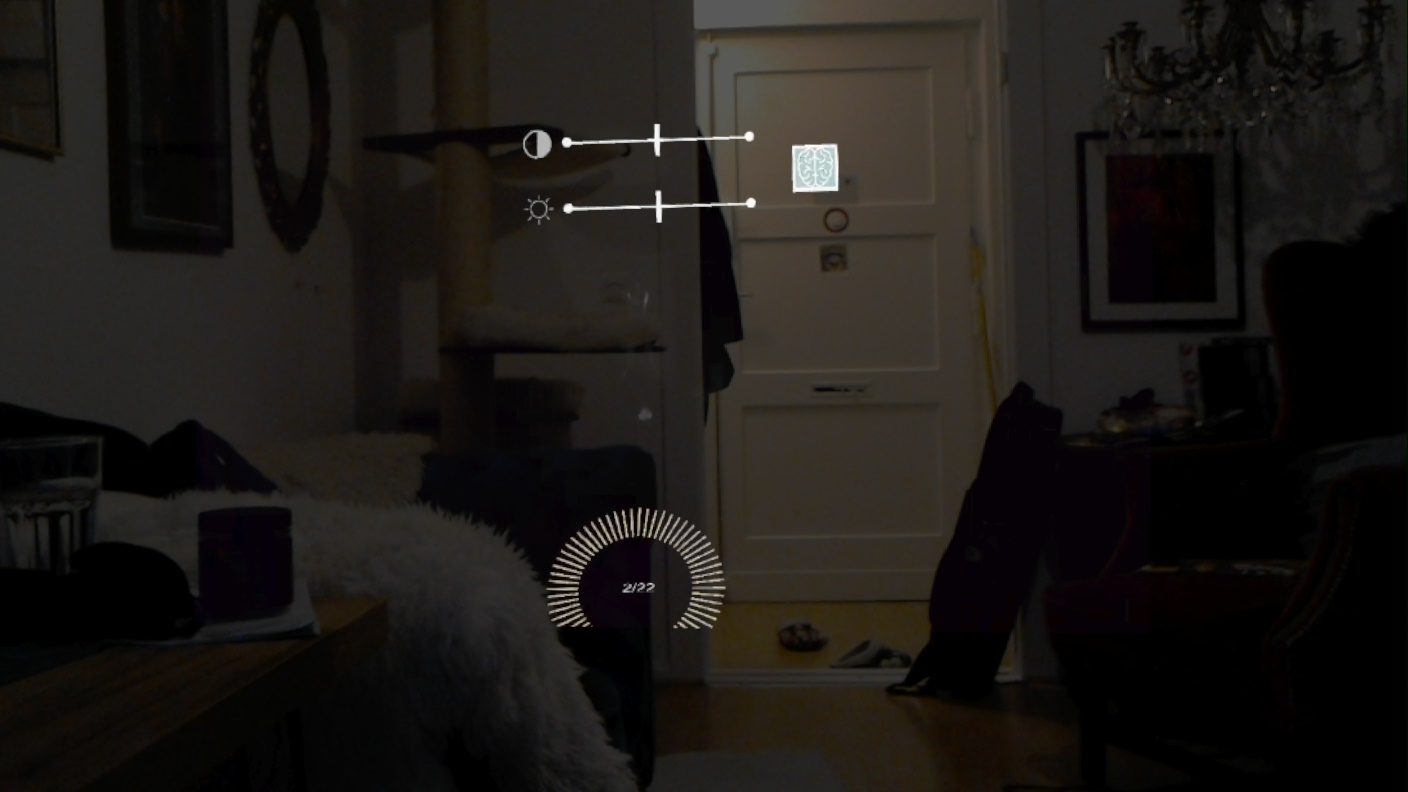
\includegraphics[width=0.5\linewidth]{images/hololens2D.jpg}
	\caption{Eine Aufnahme aus der Hololens, während die 2D-Scene von mARt dargestellt wird in einem eher dunklen Raum. Die Interaktionselemente sind gut zu erkennen, die MRT-Bilder nicht.}
	\label{img:ARLicht}
	\source{Eigene Darstellung}
\end{figure}
\FloatBarrier

Ein weiterer Punkt, der die Verwendung der Anwendung auf der Hololens erschwert ist das eingeschränkte Sichtfeld des Gerätes. Die Größe des Bereich im Sichtfeldes des Nutzers, in dem die Hololens augmentierte Inhalte darstellen kann wurde im Kapitel \ref{grundlagen} demonstriert. 
Die Begrenzung der Darstellung führt dazu, dass die MRT-Daten aus der Sicht des Nutzers meist abgeschnitten sind. Um die Daten gleichzeitig mit den Interaktionselementen sehen zu können, muss der Nutzer einen Abstand von ca. 1,5m zur Darstellung haben. Dies macht es ihm allerdings unmöglich mit dieser zu interagieren. Um die Darstellung manipulieren zu können, muss er also zwischen MRT-Bildern und Bedienelementen hin- und herblicken. Dabei werden die virtuellen Hände des Nutzer nicht angezeigt, wenn er diese nicht direkt ansieht, auch wenn die Leap Motion diese vielleicht noch erfasst. 
Die Darstellung der Hände selbst nimmt bereits einen großen Teil des Sichtfeldes der Hololens ein, da sie sich nahe am HMD befinden. 
Eine Bedienung der Anwendung auf der Hololens ist aus diesen Gründen sehr schwer. 


